\documentclass[9pt,twocolumn,twoside,]{pnas-new}

% Use the lineno option to display guide line numbers if required.
% Note that the use of elements such as single-column equations
% may affect the guide line number alignment.


\usepackage[T1]{fontenc}
\usepackage[utf8]{inputenc}

% tightlist command for lists without linebreak
\providecommand{\tightlist}{%
  \setlength{\itemsep}{0pt}\setlength{\parskip}{0pt}}


% Pandoc citation processing
\newlength{\cslhangindent}
\setlength{\cslhangindent}{1.5em}
\newlength{\csllabelwidth}
\setlength{\csllabelwidth}{3em}
\newlength{\cslentryspacingunit} % times entry-spacing
\setlength{\cslentryspacingunit}{\parskip}
% for Pandoc 2.8 to 2.10.1
\newenvironment{cslreferences}%
  {}%
  {\par}
% For Pandoc 2.11+
\newenvironment{CSLReferences}[2] % #1 hanging-ident, #2 entry spacing
 {% don't indent paragraphs
  \setlength{\parindent}{0pt}
  % turn on hanging indent if param 1 is 1
  \ifodd #1
  \let\oldpar\par
  \def\par{\hangindent=\cslhangindent\oldpar}
  \fi
  % set entry spacing
  \setlength{\parskip}{#2\cslentryspacingunit}
 }%
 {}
\usepackage{calc}
\newcommand{\CSLBlock}[1]{#1\hfill\break}
\newcommand{\CSLLeftMargin}[1]{\parbox[t]{\csllabelwidth}{#1}}
\newcommand{\CSLRightInline}[1]{\parbox[t]{\linewidth - \csllabelwidth}{#1}\break}
\newcommand{\CSLIndent}[1]{\hspace{\cslhangindent}#1}


\templatetype{pnasresearcharticle}  % Choose template

\title{Diversité des collaborations des élèves de la 59e cohorte
d'écologie de (université de Sherbooke)}

\author[a]{Marguerite Duchesne}
\author[a]{Florian Jordan}
\author[a]{Anthony St-Pierre}
\author[a]{Simon Grégoire}
\author[a]{Francis Lessard}

  \affil[a]{Université de Sherbrooke, Départment de biologie, 2500
Boulevard de l'Université, Sherbrooke, Québec, J1K 2R1}


% Please give the surname of the lead author for the running footer
\leadauthor{}

% Please add here a significance statement to explain the relevance of your work
\significancestatement{}


\authorcontributions{}



\correspondingauthor{\textsuperscript{} }

% Keywords are not mandatory, but authors are strongly encouraged to provide them. If provided, please include two to five keywords, separated by the pipe symbol, e.g:
 \keywords{  Collaborations |  Réseau écologique |  Travaux d'équipe  } 

\begin{abstract}
Nous avons voulu nous intérésser aux collaborations des élèves de
l'Université de Sherbrooke lors de travaux d'équipe pendant leur
parcours dans le baccalauréat en biologie. Pour ce faire, nous avons
dressé un réseau reliant tous les étudiants qui ont suivi le cours de
méthodes en écologie computationnelle (BIO500) lors de la session
d'hiver 2022 et qui démontre le nombre de collaborations qui ont eu lieu
entre eux tout au long de leur parcours universitaire. Nous avons
comparé le nombre total de collaborations de chaque étudiant ainsi que
le nombre de collaborations différentes de chaque étudiant dans le but
de déterminer s'ils ont tendance à conserver les mêmes équipes ou non.
Nous avons aussi observé l'impact que le cours de méthodes analytiques
en biologie (TSB303) possédait sur le réseau puisque ce dernier comporte
un travail d'équipe de 15 personnes. Nous avions un soupçon qu'un
travail de cette ampleur modifierait beaucoup le réseau final, et à la
lumière de nos résultats, cette hypothèse a été confirmée. On peut aussi
facilement identifier sur le réseau les groupes de travail qui se sont
maintenus à travers le baccalauréat, ce qui prouve que les étudiants
n'avaient pas tendance à beaucoup diversifier leurs collaborations.
\end{abstract}

\dates{This manuscript was compiled on \today}
\doi{\url{www.pnas.org/cgi/doi/10.1073/pnas.XXXXXXXXXX}}

\begin{document}

% Optional adjustment to line up main text (after abstract) of first page with line numbers, when using both lineno and twocolumn options.
% You should only change this length when you've finalised the article contents.
\verticaladjustment{-2pt}



\maketitle
\thispagestyle{firststyle}
\ifthenelse{\boolean{shortarticle}}{\ifthenelse{\boolean{singlecolumn}}{\abscontentformatted}{\abscontent}}{}

% If your first paragraph (i.e. with the \dropcap) contains a list environment (quote, quotation, theorem, definition, enumerate, itemize...), the line after the list may have some extra indentation. If this is the case, add \parshape=0 to the end of the list environment.

\acknow{}

\hypertarget{introduction}{%
\section{Introduction}\label{introduction}}

On entend souvent l'expression « Ah que le monde est petit ! » lorsque
deux personnes se retrouvent à avoir une connexion qu'on ne suspectait
pas. Certaines études se sont intéressées à ce principe que par un lien
relativement proche, tout le monde se connaît à un certain niveau.
Milgram (1967) s'est penché sur le sujet et à testé cette hypothèse
selon laquelle deux personnes pigées au hasard devraient avoir un lien
quelconque entre eux (1). Ce principe peut s'appliquer à l'écologie, car
d'un point de vu de l'évolution, toutes les espèces sont reliées par un
ancêtre commun et pour étudier les réseaux trophiques (2). Ce modèle de
« petit monde » peut donc s'appliquer à grande et petite échelle. Nous
avons voulu tester cette théorie à très petite échelle dans le
baccalauréat de la 59e cohorte d'écologie de l'Université de Sherbrooke.
Dans l'idée que l'école forme les futurs travailleurs de demain, avoir
un grand nombre de collaborations à l'université peut être bénéfique si
on se fie aux recommandations de plusieurs firmes aidant les
travailleurs à optimiser leurs capacités communes au travail. Un réseau
de collaborations diversifié entraîne un engagement plus élevé des
employés, une meilleure rétention, une plus grande diversité et plus
d'innovation (Holtzman and Anderberg, 2011). Nous nous sommes donc posés
la question si le réseau de collaborations entre les étudiants du
baccalauréat en écologie favorisait la diversité des collaborations.
Plus spécifiquement, nous avons étudié si les élèves ont tendance à
conserver les mêmes collaborateurs dans tous les travaux ou s'ils
avaient plus tendance à diversifier leurs partenaires. En effet, il est
intéressant de voir si les étudiants ont plusieurs groupes d'amis ou si
au cours du baccalauréat, ils sont restés toujours avec les mêmes
personnes. Pour les gens pour lesquels on juge avoir un grand nombre de
collaborations, est-ce qu'il y a un moyen de trouver ce qui leur a
permis d'obtenir un grand nombre de collaborations en vue d'augmenter le
nombre de collaborations des élèves? Nous avons aussi vérifié si le
cours de méthodes analytiques en biologie (TSB303) a eu un grand effet
dans le réseau de collaborations, puisque dans ce cours, les travaux
étaient en équipe de 15. On peut donc s'imaginer qu'à lui seul, ce cours
ajoute beaucoup de collaborations entre les étudiants. Pour aider à
visualiser le tout, une première figure va détailler toutes les
collaborations entre tous les individus de la cohorte. Puis, plus
spécifiquement, une autre figure qui démontre uniquement les liens de
plus de X collaborations sera présentée et ensuite cette même figure
sera comparée, mais en excluant le cours TSB303.

\hypertarget{muxe9thode}{%
\section{Méthode}\label{muxe9thode}}

La classe de BIO500 de la session d'hiver 2022 s'est divisée en 9 (à
valider) équipes. Chaque élève de ces équipes a compilé l'ensemble des
cours réalisés lors de leur baccalauréat ainsi que les informations
considérées pertinentes reliées à ces cours dans une première table
commune à l'équipe. Ils ont également compilé dans une seconde table le
nom de chaque coéquipier, l'année de début de leur baccalauréat, le nom
de leur programme ainsi que les informations considérées pertinentes
reliées à chaque individu de l'équipe. Ils ont terminé la compilation
des données par une troisième table. Au sein de cette dernière table se
trouve l'ensemble des collaborations, c'est-à-dire l'ensemble des noms
avec qui chaque élève a réalisé des travaux d'équipe jusqu'à présent
lors de leur baccalauréat.

Une fois la compilation des données réalisée par chaque équipe, celle-ci
fut partagée et mise en commun. Maintenant indépendantes, les équipes
avaient alors la tâche de fusionner l'ensemble des données ensemble afin
de n'avoir que trois tables contenant l'ensemble des données de la
classe. Au préalable, chaque équipe a dû standardiser les données de
l'ensemble des équipes afin d'obtenir une unité structurelle au sein des
différentes tables. Ces données ont ensuite été intégrées dans le
système de gestion de données SQLite3. Afin de répondre à la question
posée, les données d'intérêt ont été extraites via des requêtes et
finalement analysées.

\hypertarget{ruxe9sultats}{%
\section{Résultats}\label{ruxe9sultats}}

Pour mieux illustrer les réponses aux questions, plusieurs figures
présenteront les liens entre les étudiants.

La figure 1 représente le réseau de toutes les collaborations depuis le
début du baccalauréat des étudiants du cours de méthodes en écologie
computationnelle (BIO500) à l'hiver 2022. La grandeur des cercles est
déterminée par le nombre collaborations de chaque élève, les cercles les
plus petits correspondant à une collaboration tandis que les plus grands
correspondent à XX collaborations.

La figure 2 est le réseau des différentes collaborations avec les
collaborations issues du cours de méthodes analytiques en biologie
(TSB303) contrasté. La grandeur des cercles est déterminée par le nombre
collaborations de chaque élève, les cercles les plus petits
correspondant à une collaboration tandis que les plus grands
correspondent à XX collaborations.

La figure 3 est le réseau des différentes collaborations depuis le début
du baccalauréat des étudiants du cours de méthodes en écologie
computationnelle (BIO500) à l'hiver 2022 possédant 30 collaborations et
plus. La grandeur des cercles est déterminée par le nombre de
collaborations de chaque élève, les cercles les plus petits
correspondant à XX collaboration tandis que les plus grands
correspondent à XX collaborations.

Notre quatrième et dernière figure représente le réseau des différentes
collaborations des étudiants, mais sans le cours TSB303 qui semble avoir
une grande influence sur le réseau. C'est donc la même figure que la 2,
mais avec les liens de TSB303 en gras.

\begin{figure}
\centering
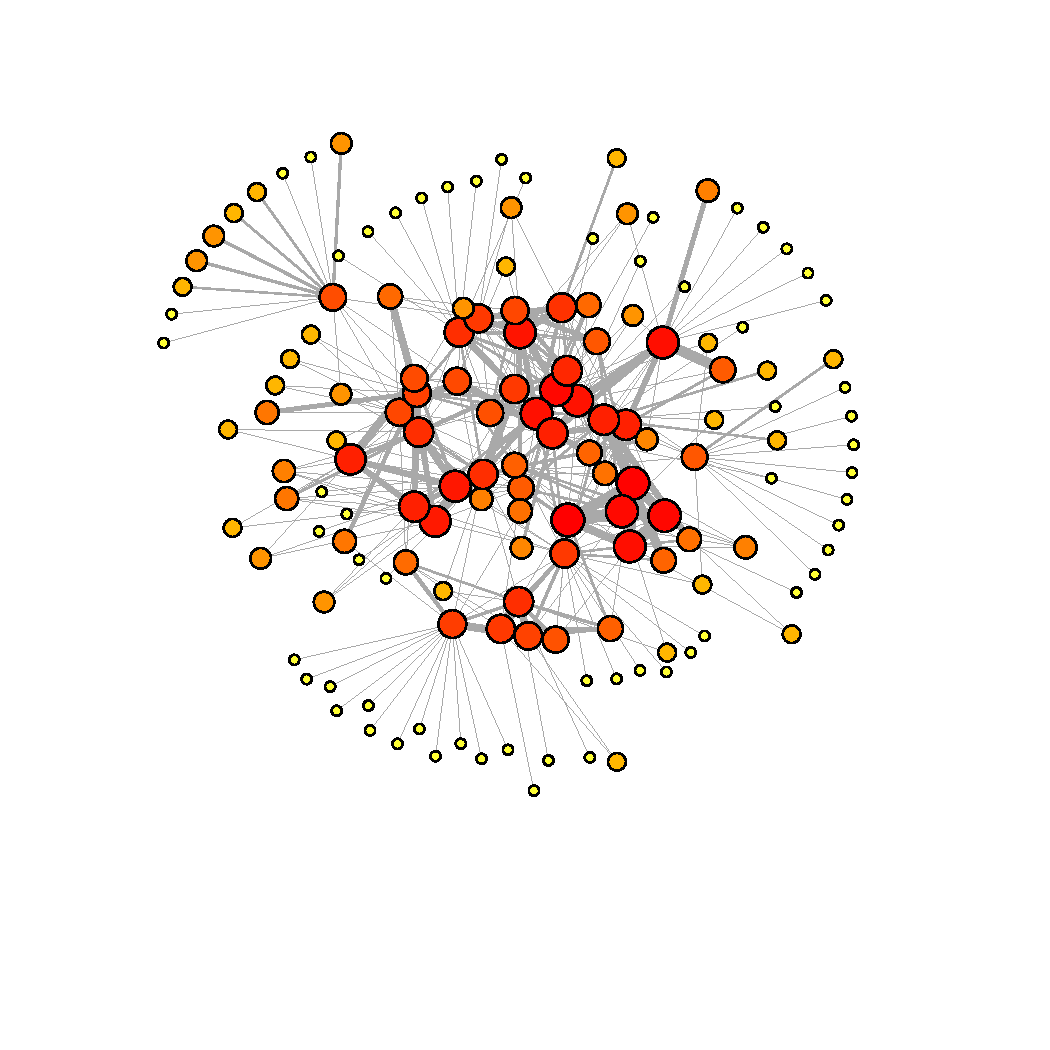
\includegraphics[width=0.5\textwidth,height=0.4\textheight]{"C:/Users/margu/Documents/Session_5/BIO500/Bio500/results/figure1.png"}
\caption{Réseaux de collaboration des étudiants de la 59e cohorte de
l'automne 2019 à l'hiver 2022. \label{fig:plot1}}
\end{figure}

\begin{figure}
\centering
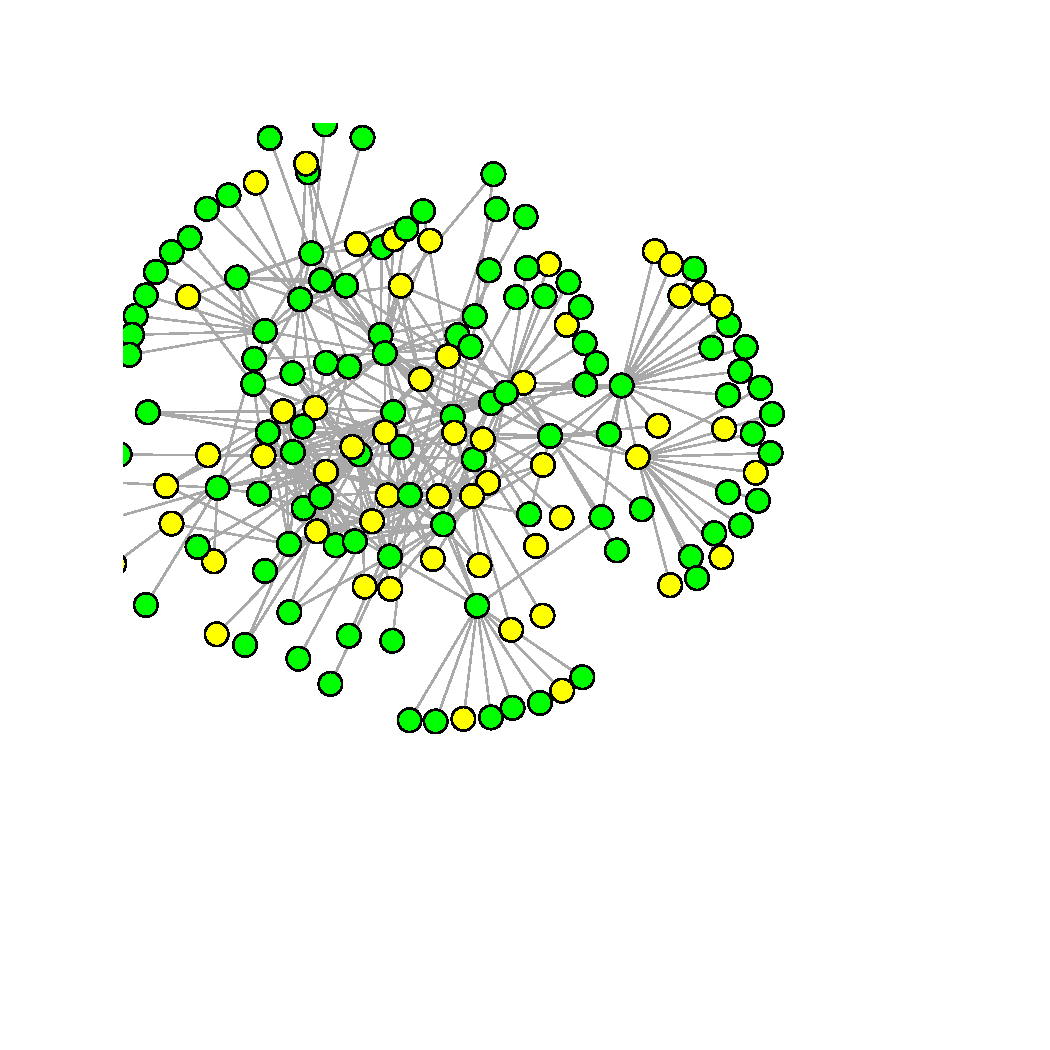
\includegraphics[width=0.5\textwidth,height=0.4\textheight]{"C:/Users/margu/Documents/Session_5/BIO500/Bio500/results/figure2.png"}
\caption{Les différentes collaborations des élèves de la 59e cohorte de
l'automne 2019 à l'hiver 2022 \label{fig:plot2}}
\end{figure}

\begin{figure}
\centering
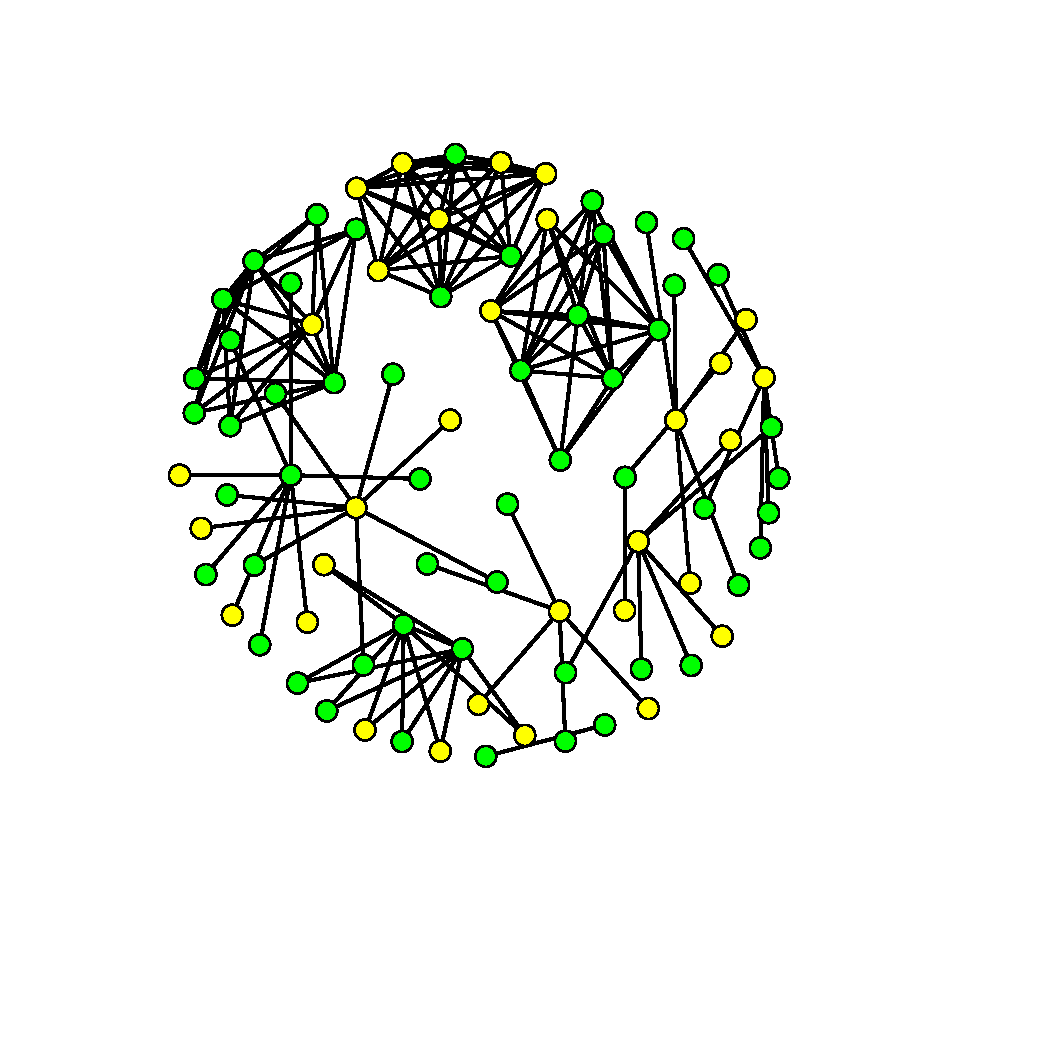
\includegraphics[width=0.5\textwidth,height=0.4\textheight]{"C:/Users/margu/Documents/Session_5/BIO500/Bio500/results/figure3.png"}
\caption{Réseau de collaborations des élèves de la 59e cohorte de
l'automne 2019 à l'hiver 2022 qui ont plus de 30 collaborations
\label{fig:plot3}}
\end{figure}

\begin{figure}
\centering
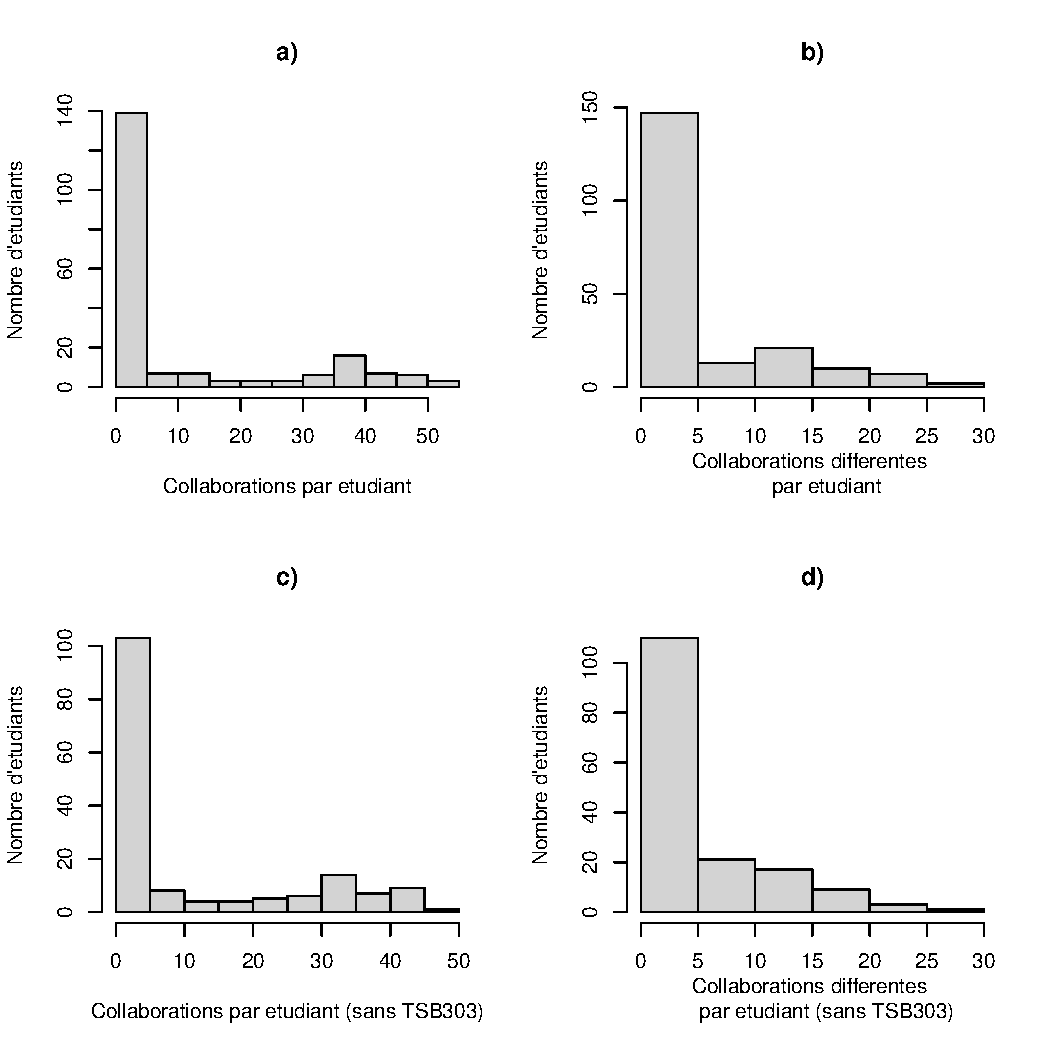
\includegraphics[width=0.5\textwidth,height=0.4\textheight]{"C:/Users/margu/Documents/Session_5/BIO500/Bio500/results/figure4.png"}
\caption{Réseau de collaborations des élèves de la 59e cohorte de
l'automne 2019 à l'hiver 2022 sans le cours TSB303 \label{fig:plot4}}
\end{figure}

\hypertarget{discussion}{%
\section{Discussion}\label{discussion}}

Rapidement, il est possible de remarquer que les élèves ont tendance à
utiliser le même réseau. Les cercles rapprochés les uns des autres
permettent de distinguer les élèves qui ont formé à plusieurs occasions
des groupes collaboratifs avec les mêmes étudiants afin d'accomplir
leurs travaux d'équipes durant leur baccalauréat. Une plus grande
diversité de collaborations aurait été visible s'il y avait eu une moins
grande ségrégation de groupes de cercles. Dans un tel cas, la figure 1
tendrait vers une homogénéité et la grosseur des cercles serait en
moyenne plus importante.

Jugeant que 30 collaborations et plus correspondaient à beaucoup de
collaborations, nous avons donc porté notre réflexion à comprendre ce
qui avait mené ces gens à obtenir autant de collaborations. Une méthode
couramment utilisée en écologie est le calcul du coefficient de Jaccard
(3) qui nous permettrait de quantifier l'hétérogénéité des interactions
par l'analyse des liens partagés. De cette manière, il serait possible
de distinguer des similarités dans la source du grand nombre de
collaborations de ces étudiants (4) et ainsi nous pourrions recommander
certaines directives aux professeurs afin d'augmenter le nombre de
collaborations des élèves.

Lorsqu'on ajoute le cours TSB303 aux collaborations, on identifie une
augmentation du nombre de collaborations. En revanche, la quantité ne
semble pas toujours être la solution pour augmenter les bienfaits de la
collaboration. En effet, il faut également mentionner la qualité des
collaborations. Un travail de moins d'une dizaine de pages réalisé par
15 personnes ne laisse pas beaucoup de marge pour que le travail soit
réparti équitablement et donc la valeur du travail d'équipe peut être
amoindri. D'autant plus que, le défi de communication entre les membres
de l'équipe est potentiellement plus grand que l'accomplissement du
travail lui-même. À terme, il semble donc justifié de ne pas comparer ce
type de collaboration aux autres où le nombre de collaborateurs pour un
travail tourne davantage autour de XX.

\hypertarget{conclusion}{%
\section{Conclusion}\label{conclusion}}

\newpage

\hypertarget{bibliographie}{%
\section*{Bibliographie}\label{bibliographie}}
\addcontentsline{toc}{section}{Bibliographie}

\hypertarget{refs}{}
\begin{CSLReferences}{0}{0}
\leavevmode\vadjust pre{\hypertarget{ref-milgram1967small}{}}%
\CSLLeftMargin{1. }
\CSLRightInline{Milgram S (1967) The small world problem.
\emph{Psychology today} 2(1):60--67.}

\leavevmode\vadjust pre{\hypertarget{ref-montoya2002small}{}}%
\CSLLeftMargin{2. }
\CSLRightInline{Montoya JM, Solé RV (2002)
\href{https://doi.org/10.1006/jtbi.2001.2460}{Small {World} {Patterns}
in {Food} {Webs}}. \emph{Journal of Theoretical Biology}
214(3):405--412.}

\leavevmode\vadjust pre{\hypertarget{ref-legendre2012numerical}{}}%
\CSLLeftMargin{3. }
\CSLRightInline{Legendre P, Legendre L (2012) Numerical ecology, 3rd
english edition, v. 24.}

\leavevmode\vadjust pre{\hypertarget{ref-delmas2019analysing}{}}%
\CSLLeftMargin{4. }
\CSLRightInline{Delmas E, et al. (2019) Analysing ecological networks of
species interactions. \emph{Biological Reviews} 94(1):16--36.}

\end{CSLReferences}



% Bibliography
% \bibliography{pnas-sample}

\end{document}
